\documentclass{ansconf}

\usepackage[T1]{fontenc}     % Use T1 encoding instead of OT1
\usepackage[bitstream-charter]{mathdesign} % Use BT Charter font
\usepackage[utf8]{inputenc}  % Use UTF8 input encoding
\usepackage{microtype}       % Improve typography
\usepackage{amsmath}         % AMS Math extensions
\usepackage{booktabs}        % Improved table spacing
\usepackage{graphicx}
\usepackage{url}
\usepackage{tikz}
\usepackage{subfigure}
\usetikzlibrary{arrows,shapes,positioning}
\usetikzlibrary{decorations.markings}
\usepackage{etoolbox}
\usetikzlibrary{matrix,calc}

\numberwithin{equation}{section}

\authorHead{Herman}
\shortTitle{4-th Order Generalized Runge-Kutta}
\confTitle{}
\confLocation{}
\confPublished{}
\lfoot{}

\begin{document}

\title{Generalized Runge-Kutta Methods for Solving Stiff Ordinary Differential Equations for Reactor Physics Applications}

\author{Bryan R. Herman}
\affil{Massachusetts Institute of Technology}

\maketitle
\thispagestyle{empty}

\Section{Introduction}

When dealing with multiple coupled ordinary first order differential equations, the question of stiffness of the system arises. The can occur when independent variables of the system are represented on different scales and their magnitudes may span many orders of magnitude. An example that we encounter in nuclear reactor analysis is the neutron kinetics equations where fluxes and precursor concentrations are calculated. Furthermore when coupling to thermal-hydraulics, a different set of physics is introduced that is represented on a different scale. Therefore, it is import to understand how to solve stiff sets of ordinary differential equations.

There are many methods that we can try and use to solve stiff sets of equations. First, we can try and use a simple explicit method. However, in this method, we must follow the equation with the shortest length scale to maintain stability of the system. If an simple implicit scheme is used, stability can be guaranteed, but we give up accuracy if we use a large time step. In this study, we wish to investigate methods that will allow us to take a larger time step, but are also relatively stable. 

In order to use large time steps, we must use a higher order time integration scheme. Here, we chose higher order generalized Runge-Kutta methods called Rosenbrock methods. These methods were first practically applied in the work of Kaps and Rentrop and thus are also referred to as Kaps-Rentrop methods. These methods are relatively simple to implement and have shown to remain reliable. Also with these methods, an automatic step size adjustment can be embedded in the algorithm. Kaps and Rentrop showed that the smallest order for which embedding a an error estimator for automatic time step size is four. This report focuses on the derivation and implementation of a fourth-order Kaps-Rentrop method with embedded third-order truncation error estimation for automatic time step size adjustment for neutron kinetics applications.

\Section{Generalized Runge-Kutta Methods}

\Subsection{Determining Runge-Kutta Coefficients}

\Subsection{Automated Time Step Size Adjustment}

\Subsection{Implementation of 4-th Order GRK Algorithm}

\Section{Point Kinetics Equations}

The simplest reactor physics model to apply GRK to is the Point Kinetics Equations (PKE). These equations are simple zero dimensional equations where the physics of the reactor are represented through simple parameters. The derivation of the PKE are described in Appendix \ref{app:pkes}. They are 
\begin{equation} \label{eq:pkeP}
\frac{d}{dt}P\left(t\right) = \frac{\rho\left(t\right)-\beta}{\Lambda}P\left(t\right) + \sum_i\lambda_iC_i\left(t\right)
\end{equation}
and
\begin{equation} \label{eq:pkeC}
\frac{d}{dt}C_i\left(t\right) = \frac{\beta_i}{\Lambda}P\left(t\right) - \lambda_iC_i\left(t\right).
\end{equation}
Using Equations \eqref{eq:pkeP} and \eqref{eq:pkeC} the derivative vector can be created as
\begin{equation}
\frac{d}{dt}\left[\begin{array}{c}
P\left(t\right) \\
C_i\left(t\right)
\end{array} \right] = \left[ \begin{array}{c}
\frac{\rho\left(t\right)-\beta}{\Lambda}P\left(t\right) + \sum_i\lambda_iC_i\left(t\right) \\
\frac{\beta_i}{\Lambda}P\left(t\right) - \lambda_iC_i\left(t\right)
\end{array}
\right].
\end{equation}
The corresponding Jacobian matrix for this model is written as 
\begin{equation}
\mathbb{J} = \left[ \begin{array}{ccccc}
\frac{\rho\left(t\right)-\beta}{\Lambda} & \lambda_1 & \lambda_i & \hdots & \lambda_I \\
\frac{\beta_1}{\Lambda} & -\lambda_1 \\
\frac{\beta_i}{\Lambda} & & -\lambda_i \\
\vdots & & & \ddots \\
\frac{\beta_I}{\Lambda} & & & & -\lambda_I \\
\end{array} \right]
\qquad
\frac{d\mathbf{f}}{dt} = \left[ \begin{array}{c} \frac{P\left(t\right)}{\Lambda}\frac{d\rho}{dt} \\
0 \\
0 \\
0 \\
0
\end{array} \right].
\end{equation}

This model was coded up and interfaced with the GRK solver. The simplest case to run is PKE with a constant reactivity insertion. Therefore, the derivative of the reactivity will be zero. The power shape from this case is shown in Figure \ref{fig:pk_rho_const_power}. As expected, there is a prompt jump immediately in the power and then an asymptotic exponential increase persists.  It is also very important to look at the rate at which the power converges in time to confirm that the method is 4th order. A convergence plot is shown in Figure \ref{fig:pk_rho_const_order}.
\begin{figure} 
\centering 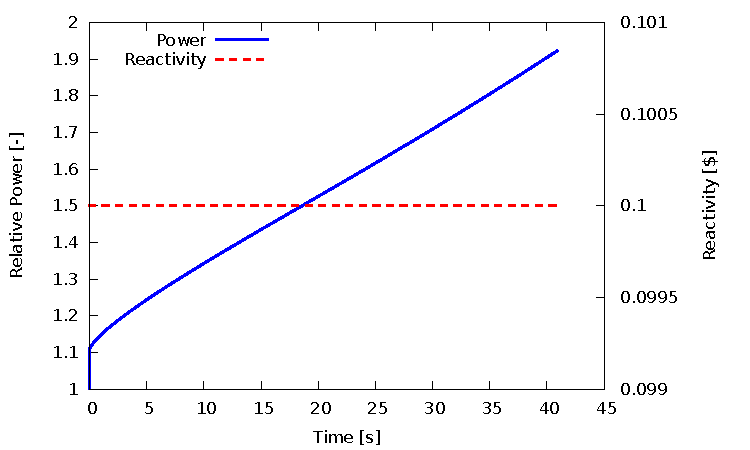
\includegraphics[scale=1.00]{./figs/pk_rho_const_power.pdf}
\caption{PKE relative power from constant reactivity insertion.}
\label{fig:pk_rho_const_power}
\end{figure}
\begin{figure} 
\centering 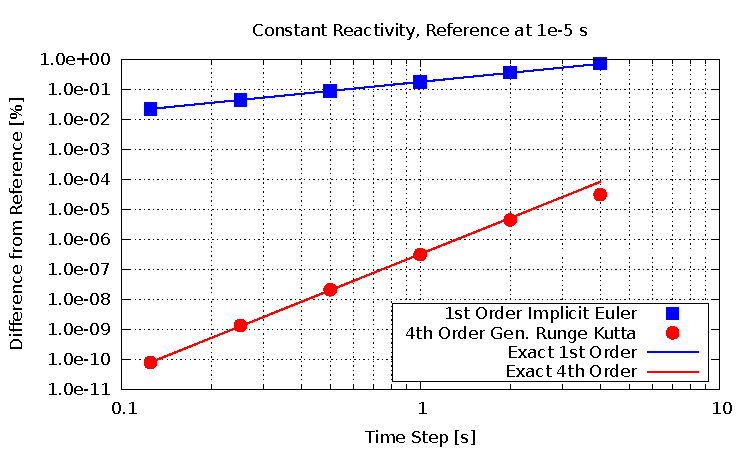
\includegraphics[scale=1.00]{./figs/pk_rho_const_order.pdf}
\caption{PKE temporal convergence rate for constant reactivity insertion.}
\label{fig:pk_rho_const_order}
\end{figure}
Two convergence rate results are shown in the plot. The first shows first order convergence of backward Euler and the second verifies 4th order convergence rate of the implemented GRK algorithm.  The reference was taken to be the GRK results at a time step of 1e-5 seconds at the end of the transient. It is also observed that the error in the GRK scheme is orders of magnitude less than backward Euler.

The next example for PKE is a case with a linear ramp reactivity insertion. This is different than the last example in that there is now a constant $\frac{d\mathbf{f}}{dt}$ term. This term is known exactly and has the slope of the reactivity ramp in it. The results of this case are shown in Figure \ref{fig:pk_rho_ramp_power}. The power looks to be the correct shape for this transient. A convergence rate test was generated again. Again, the reference is a time step of 1e-5 seconds at the end of the transient.  The results, shown in Figure \ref{fig:pk_rho_ramp_order}, show that close to 4-th order is achieved as the time step is reduced. However, numerical precision error may start to occur around 1e-10\% difference and so 4-th order is never really observed.
\begin{figure} 
\centering 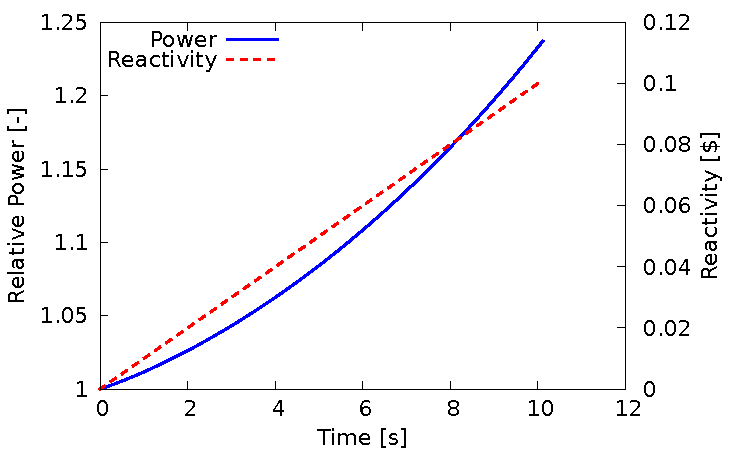
\includegraphics[scale=1.00]{./figs/pk_rho_ramp_power.pdf}
\caption{PKE relative power from ramp reactivity insertion.}
\label{fig:pk_rho_ramp_power}
\end{figure}
\begin{figure} 
\centering 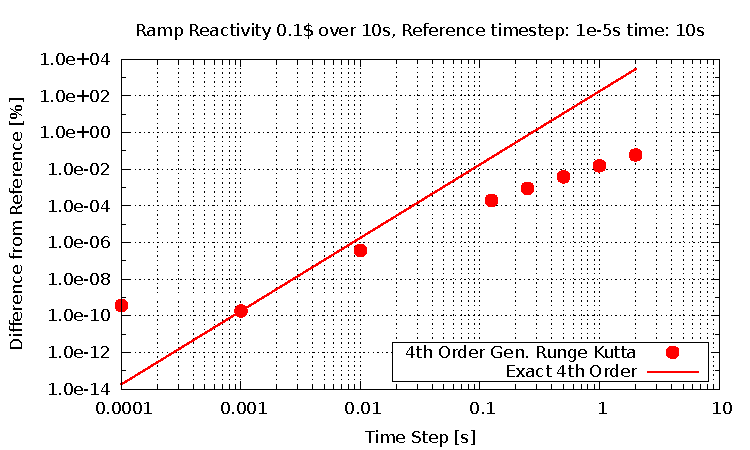
\includegraphics[scale=1.00]{./figs/pk_rho_ramp_order.pdf}
\caption{PKE temporal convergence rate for constant reactivity insertion.}
\label{fig:pk_rho_ramp_order}
\end{figure}

\Subsection{Nordheim-Fuchs Model}

The simplest reactor physics example with nonlinear feedback is the Nordheim-Fuchs model (NFM). This model couples simplified point kinetics equations with an adiabatic heat up model. It assumes that the transient occurs very quickly such that there are no delayed neutron effects. Furthermore, feedback from Doppler effect occurs instantaneously in the fuel.  The coupled set of ordinary differential equations are as follows:
\begin{equation}
    \frac{d}{dt}P\left(t\right) = \frac{\rho\left(t\right)-\beta}{\Lambda}P\left(t\right)
\end{equation}
and
\begin{equation}
    \frac{d}{dt}T_f\left(t\right) = \frac{1}{m_fc_f}P\left(t\right).
\end{equation}
The Nordheim-Fuchs model allows for a step reactivity insertion and Doppler feedback in the fuel. The reactivity model is 
\begin{equation}
    \rho\left(t\right) = \rho_0 - \alpha_f\left[T_f\left(t\right) - T_{f,0}\right].
\end{equation}
This equation shows the nonlinearity of the system of equations. Therefore, the fuel temperature must be known to get the reactivity correct and to get the fuel temperature, the reactivity must be known. The GRK scheme accounts for some of this nonlinearity in its Jacobian. The derivative vector and Jacobian for this model is
\begin{equation}
    \frac{d}{dt}\left[\begin{array}{c}
                        P\left(t\right) \\
                        T_f\left(t\right)
                      \end{array}\right] =
                \left[\begin{array}{c}
                        \frac{\rho_0 - \alpha_f\left(T_f\left(t\right) - T_{f,0}\right) - \beta}{\Lambda}P\left(t\right) \\
                        \frac{1}{m_fc_f}P\left(t\right)
                      \end{array}\right]
\end{equation}
and
\begin{equation}
    \mathbb{J} = \left[\begin{array}{cc}
                         \frac{\rho_0 - \alpha_f\left(T_f\left(t\right) - T_{f,i}\right) - \beta}{\Lambda} & -\frac{\alpha_f}{\Lambda}P\left(t\right) \\
                         \frac{1}{m_fc_f} & 0
                       \end{array}\right]
     \qquad
     \frac{d\mathbf{f}}{dt} = \left[\begin{array}{c}
                        0 \\
                        0 \\
                        \vdots
                      \end{array}\right]
\end{equation}
What is important about the NFM is that it has an analytical solution. If we define parameter $\omega$ to be
\begin{equation}
	\omega = \frac{\rho_0-\beta}{\Lambda},
\end{equation}
then the time dependence of power, fuel temperature and reactivity are as follows:
\begin{equation}
	P\left(t\right) = \frac{\Lambda\omega^2m_fc_f}{2\alpha}\mathrm{sech}^2\left(\frac{\omega t}{2}\right),
\end{equation}
\begin{equation}
	T_f\left(t\right) = \frac{\Lambda\omega}{\alpha}\mathrm{tanh}\left(\frac{\omega t}{2}\right) + T_f\left(0\right)
\end{equation}
and
\begin{equation}
	\rho\left(t\right) = \rho\left(0\right) - \left(\rho_0 - \beta\right)\mathrm{tanh}\left(\frac{\omega t}{2}\right).
\end{equation}

Results from GRK are compared to this analytical model to verify that the code is accurate.  This comparison is depicted in Figure \ref{fig:nordheim_fuchs}.
\begin{figure} 
\centering 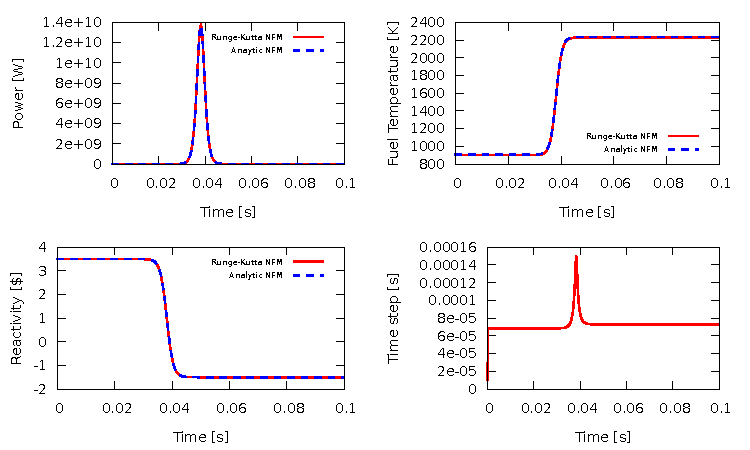
\includegraphics[scale=1.00]{./figs/nordheimfuchs.pdf}
\caption{Comparison of GRK code to Nordheim Fuchs Model.}
\label{fig:nordheim_fuchs}
\end{figure}
From the results, it is observed that GRK does very well when comparing to NFM. For the first time, the time step used as a function of time is reported. More results with variable time step will be discussed in Sections \ref{sec:1D} and \ref{sec:2D}. Before the first time step, the user supplied the code with a 1e-5 second time step. The GRK variable time step algorithm quickly noticed that this was too fine and coarsened it to about 6.5e-5 seconds. This is held fairly constant as the transient progress until feedback begins to take over. The change in the flux rapidly becomes less and less and so the time step is allowed to coarsen. This occurs until the flux quickly drops once feedback dominates and it quickly returns to its previous steady value.

\Subsection{Point Kinetics with Feedback}

It is often questioned whether an algorithm retains its order of convergence when nonlinearities are present. The NFM presented in the previous section was extended to include delayed neutron effects, energy deposition to coolant, and heat transfer between fuel and coolant.  Coolant flow through the core is also simulated. The set of coupled equations used will be described below. Terms highlighted in {\color{red} red} represent parameters that are input into the model.  The equations are:
  \begin{itemize}
    \item Equation for power (parameters in {\color{red}red} are inputs):
  \end{itemize}
  \begin{equation}
    \frac{dP}{dt} = \frac{\overbrace{{\color{red}\rho_0\left(t\right)} - {\color{red}\alpha_f}\left[T_f\left(t\right) - T_{f,0}\right] - {\color{red}\alpha_c}\left[T_c\left(t\right) - 
    T_{c,0}\right]}^{\rho\left(t\right)} - {\color{red}{\beta}}}{{\color{red}\Lambda}}P\left(t\right) + \sum_i{\color{red}\lambda_i}C_i\left(t\right),
    \label{eq:pk_power}
  \end{equation}
    \begin{itemize}
    \item Equation for precursors:
  \end{itemize}
  \begin{equation}
    \frac{dC_i}{dt} = \frac{{\color{red}\beta_i}}{{\color{red}\Lambda}}P\left(t\right) - {\color{red}\lambda_i}C_i\left(t\right),
  \end{equation}
    \begin{itemize}
    \item Equation for fuel temperature ($\xi$ is coolant power deposition fraction):
  \end{itemize}
  \begin{equation}
    \frac{dT_f}{dt} = \frac{1-{\color{red}\xi}}{{\color{red}m_fc_f}}P\left(t\right) - \frac{\color{red}hA}{\color{red}m_fc_f}\left[T_f\left(t\right) - T_c\left(t\right)\right],
  \end{equation}
    \begin{itemize}
    \item Equation for coolant temperature:
  \end{itemize}
  \begin{equation}
    \frac{dT_c}{dt} = \frac{{\color{red}\xi}}{{\color{red}m_cc_c}}P\left(t\right) + \frac{\color{red}hA}{\color{red}m_cc_c}\left[T_f\left(t\right) - T_c\left(t\right)\right]
    - \frac{2\color{red}\dot{m}}{\color{red}m_c}\left[T_c\left(t\right) - {\color{red}T_{in}}\right].
    \label{eq:pk_temp}
  \end{equation}
In Eqs. \eqref{eq:pk_power}-\eqref{eq:pk_temp}, the input variables are defined as:
\begin{itemize}
	\item $\rho_0\left(t\right)$ - time dependent input reactivity
	\item $\alpha_f$ - fuel temperature coefficient of reactivity
	\item $\alpha_c$ - coolant temperature coefficient of reactivity
	\item $\beta$ - total delayed neutron fraction
	\item $\beta_i$ - delayed neutron fraction of precursor group $i$
	\item $\Lambda$ - prompt neutron lifetime
	\item $\lambda_i$ - decay constant of precursor group $i$
	\item $\xi$ energy deposition fraction directly into coolant
	\item $m_f$ mass of fuel
	\item $m_c$ mass of coolant
	\item $c_f$ specific heat capacity of fuel
	\item $c_c$ specific heat capacity of coolant
	\item $hA$ heat transfer rate from fuel to coolant
	\item $\dot{m}$ mass flow rate of coolant
	\item $T_{in}$ inlet coolant temperature
\end{itemize}
The above equations are then placed in a derivative vector in the GRK code. The Jacobian of this model is
  \begin{equation}
    \mathbb{J} = \left[
    \begin{array}{ccccc}
      \frac{{\color{red}\rho_0\left(t\right)} - {\color{red}\alpha_f}\left[T_f\left(t\right) - T_{f,0}\right] - {\color{red}\alpha_c}\left[T_c\left(t\right) - 
    T_{c,0}\right]- {\color{red}{\beta}}}{{\color{red}\Lambda}} & \color{red}\lambda_i & \hdots & \frac{-\color{red}\alpha_f}{\color{red}\Lambda}P\left(t\right) 
    & \frac{-\color{red}\alpha_c}{\color{red}\Lambda}P\left(t\right) \vspace{0.1cm}\\
    
    \frac{{\color{red}\beta_i}}{{\color{red}\Lambda}} & -{\color{red}\lambda_i} \\
    
    \vdots & & \ddots \\
    
    \frac{1-{\color{red}\xi}}{{\color{red}m_fc_f}} & & & -\frac{\color{red}hA}{\color{red}m_fc_f} & \frac{\color{red}hA}{\color{red}m_fc_f} \vspace{0.1cm} \\
    
    \frac{{\color{red}\xi}}{{\color{red}m_cc_c}} & & & \frac{\color{red}hA}{\color{red}m_cc_c} & -\frac{{\color{red}hA} + 2\color{red}\dot{m}c_c}{\color{red}m_cc_c}
    \end{array}\right]
  \end{equation}
and
  \begin{equation}
     \frac{d\mathbf{f}}{dt} = \left[\begin{array}{c}
                        \frac{d\color{red}\rho_0}{dt}\frac{P\left(t\right)}{\color{red}\Lambda} \\
                        0 \\
                        \vdots
                      \end{array}\right].
  \end{equation}
Using this model, a rod ejection is simulated where reactivity is inserted linearly to \$1.2 over 0.2 seconds and is held constant. We expect the power to quickly rise when the rod is ejected. However, due to temperature feedback in the fuel and coolant, this abrupt power increase will be halted and a new steady state will form. Table \ref{tab:pk_feedback_input} lists all of the input variables used in this simulation.  The same eight group delayed neutron data that was used in previous analyses was used here. The initial power of the system is 5 MW. All of the other steady state values can be inferred by setting the derivatives in Eqs. \eqref{eq:pk_power}-\eqref{eq:pk_temp} to zero.
\begin{table}
\caption{Input Values used for PKE Feedback Analysis}
\label{tab:pk_feedback_input}
\centering
\begin{tabular}{cc||cc}
\toprule 
Parameter & Value & Parameter & Value\tabularnewline
\midrule
\midrule 
$\alpha_f$ & $2.5\times 10^{-5}$ 1/K & $\alpha_c$ & $25\times 10^{-5}$ 1/K \tabularnewline
\midrule 
$\xi$ & $0.05$ & $hA$ & $14633$ W \tabularnewline
\midrule 
$m_f$ & $148.3$ kg & $m_c$ & $20.4$ kg \tabularnewline
\midrule 
$c_f$ & $312$ J/kg-K & $c_c$ & $5827$ J/kg-K \tabularnewline
\midrule 
$\dot{m}$ & $24.1$ kg/s & $T_{in}$ & $559$ K \tabularnewline
\bottomrule
\end{tabular}
\end{table}

These transient was solved in the GRK code. Figure \ref{fig:pk_feedback_all} shows the results of the analysis.
\begin{figure} 
\centering 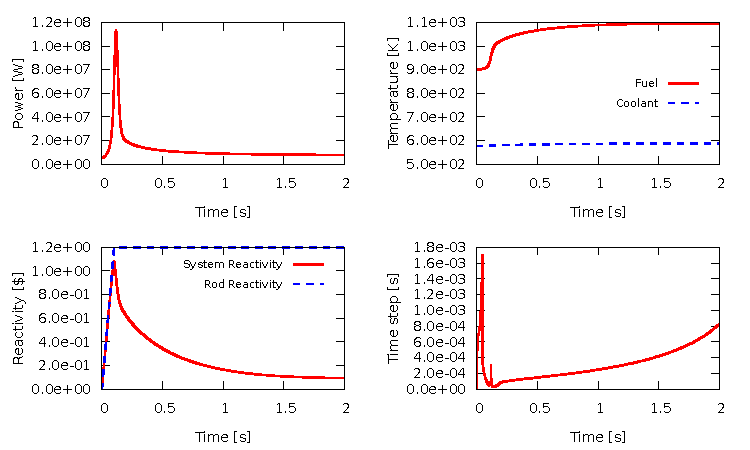
\includegraphics[scale=1.00]{./figs/pk_feedback_all.pdf}
\caption{Transient results for PKE with feedback.}
\label{fig:pk_feedback_all}
\end{figure}
As expected the power quickly rose when the rod was ejected and was limited by the temperature feedback from fuel and coolant. A plot of reactivity is also shown in the figure. Two curves are present, where the first represents the forcing function of the rod ejecting. A linear ramp is present and then held after the rod is out of the core. The second reactivity curve shown is the actual reactivity of the system.  It shows the point in time where the reactivity feedbacks from fuel and coolant start to dominate the rod reactivity insertion. The transient settles back to a different steady state as shown in the power and temperature plots.  The fuel temperature has increased by 200 K from this transient.  Finally, the variable time step behavior is shown where it coarsens and refines as appropriate.

The convergence rate of the power at different values of time is presented in Figure \ref{fig:pk_feedback_order}.
\begin{figure}
\centering 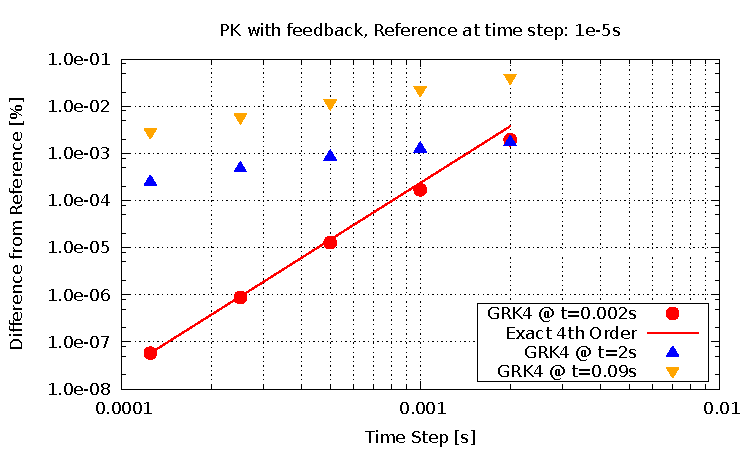
\includegraphics[scale=1.00]{./figs/pk_feedback_order.pdf}
\caption{Converge rate results for point kinetics with feedback present.}
\label{fig:pk_feedback_order}
\end{figure}
Looking at the results for 0.002 seconds, the convergence rate is nearly 4th order. However, taking the results at a later time of 0.09 seconds, the convergence rate is first order. Similarly at the end of the transient, the convergence rate remains first order. This is somewhat disconcerting since once we put nonlinear feedback in, we lose all benefit of this algorithm with respect to convergence rate. Another reason why this may occur is that there is a bug in this portion of the code, however none have been found to date.

\Section{1-D Spatial Kinetics no Feedback}\label{sec:1D}

Before analysis a 2-D reactor with local thermal feedback, significant upgrades need to made to a code. Therefore, a 1-D spatial kinetics code will be written and use basic operators to represent complex space and energy dependence such that moving to 2-D with feedback will happen naturally. With any reactor physics application, we start with the neutron balance equation. Here, we show it in 3-D multigroup steady state form over a Cartesian volume cell,
\begin{equation}
\label{eq:NBE}
\sum_{u \in x,y,z} \frac{\overline{J}^{u,g}_{l+1/2,m,n} - \overline{J}^{u,g}_{l-1/2,m,n}}{\Delta_l^u} + \overline\Sigma_{t_{l,m,n}}\overline{\overline{\phi}}_{l,m,n}^g = \sum_{h=1}^G\upsilon\overline\Sigma^{h\rightarrow g}_{s_{l,m,n}}\overline{\overline{\phi}}_{l,m,n}^h + \frac{\chi_{l,m,n}^g}{k}\sum_{h=1}^G\nu\overline\Sigma^{hg}_{f_{l,m,n}} \overline{\overline{\phi}}_{l,m,n}^h.
\end{equation}
The notation used in Eq. \eqref{eq:NBE} is as follows:
\begin{itemize}
	\item $u$ - primary direction, either $x$, $y$ or $z$,
	\item $l$ - spatial index corresponding to direction $u$,
	\item $m$ and $n$ - spatial indices of transverse directions $v$ and $w$,
	\item $g$ - energy group
	\item $h$ - energy group (dented for outgoing groups during energy transfer)
	\item $\overline{J}^{u,g}_{l\pm1/2,m,n}$ - net neutron current in on positive/negative face $l\pm1/2$ in direction $u$ and group $g$,
	\item $\Delta^u_l$ is the length of the cell in direction $u$,
	\item $\overline\Sigma_{t_{l,m,n}}$ is the cell-averaged macroscopic total cross section,
	\item $\overline{\overline{\phi}}_{l,m,n}^g$ is the cell-averaged neutron flux,
	\item $\upsilon\overline\Sigma^{h\rightarrow g}_{s_{l,m,n}}$ is the cell-averaged macroscopic neutron production scattering cross section (includes n,$x$n reactions) transferring from group $h$ to group $g$,
	\item $\chi_{l,m,n}^g$ total fission emission spectrum into group $g$,
	\item $k$ is the core multiplication factor,
	\item $\nu\overline\Sigma^{h}_{f_{l,m,n}}$ is the macroscopic neutron production fission cross section.
\end{itemize}
 We will apply the diffusion approximation to relate neutron current to flux. This approximation known as Fick's Law is
 \begin{equation}
     \overline{J}^{u,g}_{l\pm1/2,m,n} = -D_{l,m,n}^g\left.\frac{d\overline{\phi}^g}{du}\right|_{l\pm 1/2,m,n},
 \end{equation}
where $D_{l,m,n}^g$ is the diffusion coefficient and $\overline{\phi}^g$ is the group $g$ neutron flux averaged over the transverse area in directions $v$ and $w$. This equation is then discretized using mesh-centered finite difference methods. The derivation of the subsequent equation is detailed thoroughly in Appendix \ref{app:fdm}. Relations are shown for two cases:
\begin{itemize}
	\item cell-to-cell coupling
	\begin{equation}
	    \overline{J}^{u,g}_{l\pm1/2,m,n} = \frac{2D_{l\pm1,m,n}^gD_{l,m,n}^g}{D_{l\pm1,m,n}^g\Delta_l^u + D_{l,m,n}^g\Delta_{l\pm1}^u}\overline{\overline{\phi}}_{l,m,n}^g,
	\end{equation}
	\item cell-to-boundary coupling
	\begin{equation}
	    \overline{J}^{u,g}_{l\pm1/2,m,n} = \pm\frac{2D_{l,m,n}^g\left(1 - \beta_{l\pm1/2,m,n}^g\right)}{4D_{l,m,n}^g\left(1 + \beta_{l\pm1/2,m,n}^g\right) + \left(1 - \beta_{l\pm1/2,m,n}^g\right)\Delta_l^u}\overline{\overline{\phi}}_{l,m,n}^g.
	\end{equation}
\end{itemize}
The only new parameter not defined in these equations is the surface albedo, $\beta_{l\pm1/2,m,n}^g$ which is the ratio of incoming to outgoing partial neutron current. Therefore for reflective boundary conditions the albedo is 1.0, zero incoming current it is 0.0 and for zero flux it is -1.0.

An neutron balance equation with diffusion approximation can be written for each cell and energy group creating a linear system of equations. In steady state form, these coupled system of equations can be represented in operator form as
\begin{equation}\label{eq:steady_oper}
    \mathbb{M}\boldsymbol{\Phi} = \frac{1}{k}\mathbb{F}\boldsymbol{\Phi},
\end{equation}
where $\mathbb{M}$ represents the loss of neutrons and $\mathbb{F}$ represents the production of neutrons from fission. Note, this equation is a generalized eigenvalue problem. Therefore a suitable eigenvalue solver must be available to solve for the steady state flux shape and multiplication factor $k$.

After getting the steady state values, the transient diffusion equations or spatial kinetics equations can be solved. We can write the neutron balance equation from Eq. \eqref{eq:NBE} in time-dependent form as
\begin{align}
\label{eq:time_NBE}
\left(\frac{1}{v}\right)_{l,m,n}^g\frac{\partial}{\partial t}\overline{\overline{\phi}}_{l,m,n}^g + \sum_{u \in x,y,z} \frac{\overline{J}^{u,g}_{l+1/2,m,n} - \overline{J}^{u,g}_{l-1/2,m,n}}{\Delta_l^u} + \overline\Sigma_{t_{l,m,n}}\overline{\overline{\phi}}_{l,m,n}^g  & = \sum_{h=1}^G\upsilon\overline\Sigma^{h\rightarrow g}_{s_{l,m,n}}\overline{\overline{\phi}}_{l,m,n}^h \\ + \frac{\chi_{l,m,n}^{p,g}\left(1-\beta\right)}{k}\sum_{h=1}^G\nu\overline\Sigma^{hg}_{f_{l,m,n}}  \overline{\overline{\phi}}_{l,m,n}^h + \sum_i\chi_{i_{l,m,n}}^{d,g}\lambda_i C_{i_{l,m,n}}\nonumber.
\end{align}
Note that in Eq. \eqref{eq:time_NBE} all of the macroscopic cross sections may be time-dependent. Since we added time dependence back, we must include the delayed neutron precursors, which have their own separate balance equation (shown later). If we make some simple assumptions we can write this in similar operator form as above. The first assumption is that the delayed fission spectrum is independent of precursor groups and that it is equivalent to the prompt neutron spectrum. This assumption will be fine for the cases in this work, but may not be applicable to all problems.

We can write this in operator notation similar to Eq. \eqref{eq:steady_oper},
\begin{equation}
    \left(\boldsymbol{\frac{1}{v}}\right)\frac{d}{dt}\boldsymbol{\Phi} + \mathbb{M}\boldsymbol{\Phi} = \frac{1}{k}\mathbb{F}\boldsymbol{\Phi}.
\end{equation}
After spatial discretization, the equation becomes an ordinary differential equation. This can be directly used in the GRK code. Note that the transient will be started off the steady state solution that includes $\boldsymbol{\Phi}$ and $k$.  The multiplication factor, which balances production and destruction of neutrons at steady state, must be held constant throughout the transient.

\Section{2-D LRA Benchmark}\label{sec:2D}

\Section{Conclusion}

\setlength{\baselineskip}{12pt}

\bibliographystyle{ans}
\bibliography{references}

\appendix

\section{Nonautonomous Form of Generalized Runge-Kutta}

\section{Derivation of Order Equations}

\section{Derivation of Point Kinetics Equations} \label{app:pkes}

\section{Mesh-centered Finite Difference Equations} \label{app:fdm}

\end{document}